\section{Introduction}
\label{sec:intro}

Output preconditioning can improve a Muon optimizer that already whitens its inputs. The useful approximation depends on the projection: large MLP expansion outputs admit cheap coordinate scaling, while smaller residual-stream outputs benefit from dense factors that capture cross-channel structure. This distinction makes the second side practical. All-diagonal output factors (OD-All) give little or no held-out gain at 130M and fall behind MuonT when model width doubles, consistent with this distinction.

Muon maps matrix momentum toward a semi-orthogonal update using Newton--Schulz iterations~\citep{jordan2024muon}. MuonT, also called Toner, adds input activation moments around this map and improves pretraining loss~\citep{mohamadi2026toner}. For a linear layer $y=Wx$, however, the gradient $G=\sum_j\delta_jx_j^{\Tr}$ depends on both the forward activation $x_j$ and the output cotangent $\delta_j=\partial\ell/\partial y_j$. Input-only whitening uses one of these two signals. We ask whether the second moment of $\delta$ provides an additional benefit after input whitening, and what it costs to use it.

A symmetric formula does not imply symmetric computational needs. In the Transformers we study, the two expanded MLP outputs account for 96.2\% of nominal output eigendecomposition work, yet most of their anisotropy is diagonal. The outputs that write back into the residual stream are much smaller, but their unequal eigenvalues are almost invisible in coordinate second moments. Dense input factors remain useful even at expansion width. Output factors also arrive later in the step and require frequent eigenbasis repairs, making their scheduling a separate problem from input preconditioning.

\begin{figure}[t]
  \centering
  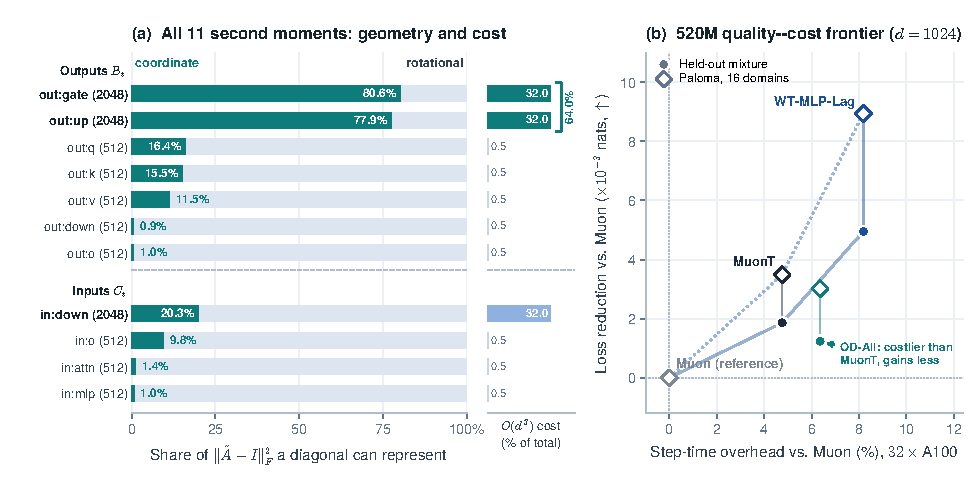
\includegraphics[width=\textwidth]{fig1_overview.pdf}
  \caption{\textbf{Output geometry suggests where dense preconditioning is worth its cost.}
  \textbf{(a)} Diagonal and off-diagonal shares of anisotropy for all 11 moments (130M, Muon trajectory, step 2,500). Each bar shows the 32-layer median of $\mathrm{DiagAniso}$ from \cref{eq:diag_aniso} and its complement, $1-\mathrm{DiagAniso}$. The split describes where anisotropy lies in the model's coordinate basis; it does not show its total magnitude. The cost column gives each moment's share of nominal dense eigendecomposition work across all 11 moments; teal marks the two moments WT-MLP-Lag diagonalizes. Expanded outputs have mostly diagonal anisotropy and account for 96.2\% of output-side cubic work; the equally wide \texttt{down} input retains cross-channel structure.
  \textbf{(b)} Final held-out and Paloma gains versus Muon at 520M, against median step-time overhead on 32 A100 GPUs. WT-MLP-Lag extends MuonT's quality gain with an incremental throughput cost. This run uses one seed.}
 \label{fig:overview}
\end{figure}

We build \mname{WT-MLP-Lag} around these observations. It retains MuonT's dense input factors, uses dense output factors at hidden width, and uses diagonal output factors on the expanded \texttt{gate} and \texttt{up} projections. A one-update lag lets the output reduction and root solver overlap the next training step. The mathematical approximation removes most of the nominal cubic output work; asynchronous execution reduces the exposed latency that remains.

The resulting gains survive three tests: fresh paired seeds at 130M, four times as many training tokens, and transfer to 520M without retuning the output-side recipe (\Cref{fig:scaling_traj}). Matched-path identity controls and full-budget learning-rate sweeps reduce two sources of misleading optimizer comparisons. Counterfactual updates then test how the method changes the direction and norm of the step. Together these experiments support a practical design rule: preserve dense output geometry where channel correlations dominate, and approximate it where coordinate energy carries most of the signal.

Our evidence covers models up to 537M non-embedding parameters. It establishes a fixed-token quality improvement; the systems measurements retain a throughput penalty, and the longer and wider training comparisons still need multi-seed replication.
